\chapter{Introduction}
This thesis has two foci, both in the area of biomembranes.
One focus is on the interaction of a biomedically important Tat peptide with 
membranes.
The other is on a fundamental problem regarding the enigmatic structure of a
pure lipid bilayer.
Sec.~\ref{sec:lipid_bilayer} introduces lipid molecules that constitute
biomembranes and three thermodynamic phases displayed by lipids pertinent to this 
thesis.
The Tat peptide and its biomedical importance are introduced in Sec.~\ref{sec:Tat_peptide},
followed by a brief overview of the ripple phase in Sec.~\ref{sec:ripple_phase}.


\section{Lipid bilayer}\label{sec:lipid_bilayer}
Membranes define the boundary between living cells
and their surrounding environment. They help regulate inter- and intracellular
transport. Cell membranes are composed of lipid bilayers.
Lipid bilayers are a self-assembled system of lipids, which are 
amphiphilic molecules that consist of a hydrophilic headgroup
and hydrophobic chains (Fig.~\ref{fig:lipid}).

\begin{figure}
  \centering
  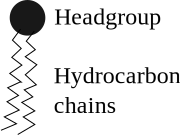
\includegraphics[width=0.2\textwidth]{figures/lipid}
  \caption{Schematic representation of a lipid molecule}
  \label{fig:lipid}
\end{figure}

In water, lipids self-assemble into lipid bilayers to shield their hydrophobic 
chains, and display a wide variety of thermodynamic phases
as a function of temperature and hydration. Figure~\ref{fig:phase_diagram}
shows a phase diagram of dimyristoylphosphatidylcholine (DMPC).
PC lipids constitute a substantial fraction of cell membranes
and have been studied for many decades \cite{Nagle00}.
At full hydration (100\% relative humidity), a lamellar phase coexists with excess water.
In the high temperature, fluid $L_\alpha$ phase, the hydrocarbon chains 
are conformationally disordered, and intra-membrane molecular correlations 
are liquid-like \cite{ref:Fahey78} (Fig.~\ref{fig:various_phases}).
The disordering of fluid phase membranes allows proteins to 
interact with cell membranes in various ways, rendering biological systems
highly complex. 
This phase is usually considered the most biologically relevant.

\begin{figure}[htbp]
  \centering
  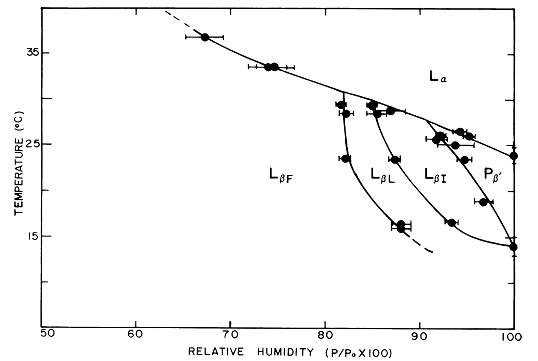
\includegraphics[width=0.9\textwidth]{figures/smith_phase_diagram}
  \caption{Experimental phase diagram of DMPC~\cite{ref:Smith88}.
  \LbetaI, \LbetaL, and \LbetaF\ belong to the gel $L_{\beta'}$ phase. $P_{\beta'}$ is 
  the ripple phase, and $L_\alpha$ is the fluid phase.}
  \label{fig:phase_diagram}
\end{figure}

\begin{figure}[htbp]
  \centering
  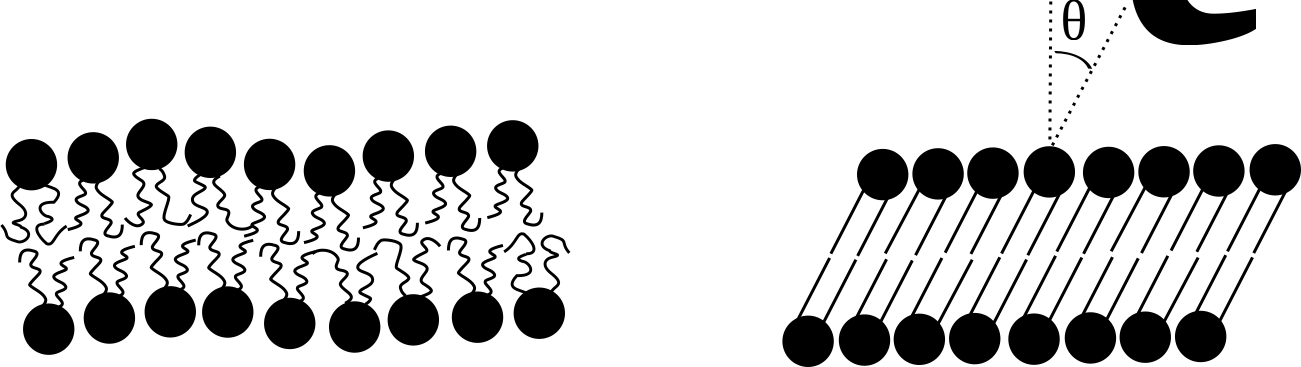
\includegraphics[width=0.9\textwidth]{figures/various_phases}
  \caption[]{Schematics of the structure of fluid $L_\alpha$ phase (left) and 
  gel $L_{\beta'}$ phase (right). Black solid circles are lipid headgroups 
  and solid lines are lipid chains. $\theta$ is the chain tilt angle.}
  \label{fig:various_phases}
\end{figure}

In the low temperature, gel $L_{\beta'}$
phase, hydrocarbon chains are stiff and tilted with respect to the membrane
normal \cite{ref:Tardieu73}, and are organized in either a hexagonal 
or orthorhombic lattice. 
The $L_{\beta'}$ is further categorized into three phases according to the 
chain tilt direction \cite{ref:Smith88,ref:Tristram93,Tristram-Nagle02}. 
In the \LbetaI\ phase, chains are tilted toward the 
nearest neighbor as shown in Fig.~\ref{fig:gel_phase_packing}, and
in the \LbetaF\ phase, chains are tilted toward the next nearest neighbor.
In the \LbetaL\ phase, chains are tilted toward an intermediate direction
between nearest and next nearest neighbors.

\begin{figure}[htbp]
  \centering
  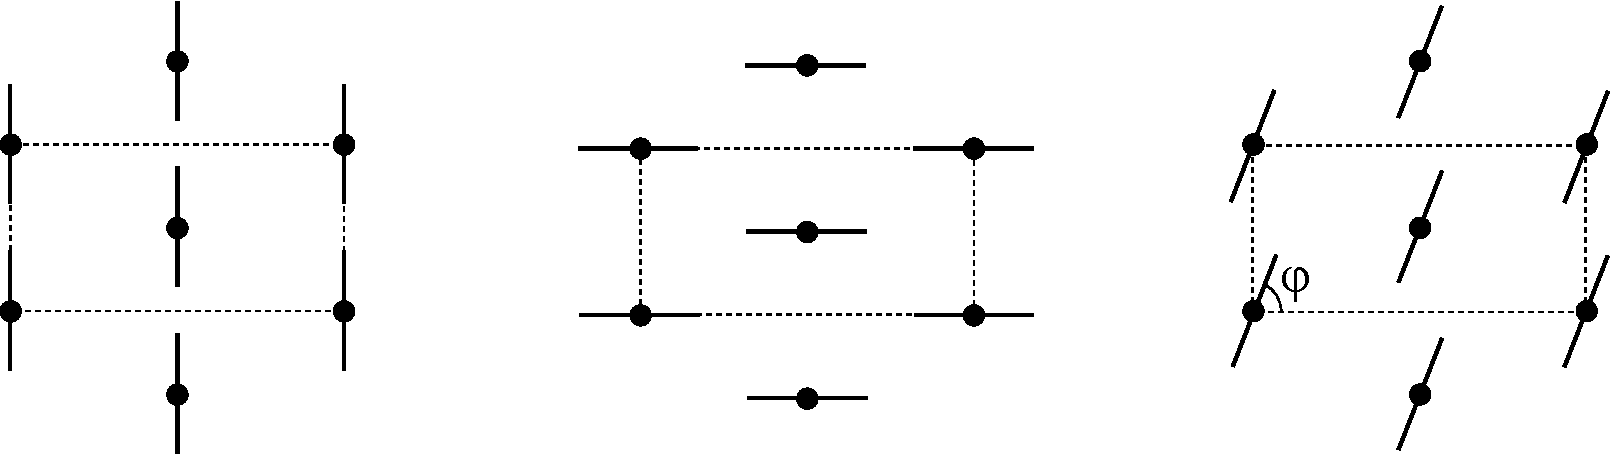
\includegraphics[width=0.9\textwidth]{figures/gel_phase_packing}
  \caption{Gel phase chains projected onto the bilayer plane showing 
  the chain tilt direction in \LbetaI\ (left), \LbetaF\ (middle), and
  \LbetaL\ (right) phases. Black dots are orthorhombic lattice points.
  Unit cells are shown in dashed lines.
  Chains are drawn as solid lines. Chains are tilted toward the
  nearest neighbor in \LbetaI\ phase with $\phi=\pi/2$. 
  In the \LbetaF\ phase, the chains are tilted toward the next nearest neighbor
  ($\phi=0$). In the \LbetaL\ phase, $0 \leq \phi \leq \pi/2$.}
  \label{fig:gel_phase_packing}
\end{figure}

There are various kinds of lipids. 
They can be 
categorized in terms of headgroup, chain saturation, and chain length.
The most studied headgroup is phosphatidylcholine (PC),
consisting of phosphate and choline groups. 
Lipid hydrocarbon chains can have one or more double bonds. 
Lipids
with no double bonds in the chains are called saturated lipids,
such as DMPC (see Fig.~\ref{fig:lipid_structure}) and DPPC. 
Lipids with one double bond
are called mono-unsaturated lipids, such as DOPC shown in Fig.~\ref{fig:lipid_structure}.
Unsaturation leads to packing frustration and lowers the melting 
temperature. For example, DOPC forms a $L_{\alpha}$ fluid phase at room temperature
while DPPC is in a $L_{\beta'}$ gel phase.
In mammalian cells, most lipids have at least one unsaturated chain.
Membrane curvature
has interested many physicists. Phosphatidylethanolamine (PE) is a small 
headgroup, and packing of PE lipids leads to spontaneous membrane curvature.
The chemical structure of DOPE is shown in Fig.~\ref{fig:lipid_structure}.
Many proteins have been found to sense/induce membrane curvature, 
making PE lipids especially attractive for those studies (REF).
Another class of headgroup is
anionic, phosphatidylserine (PS). In cells, electrostatic interactions
significantly influence biological processes and naturally occurring anionic
lipids have been the focus of many studies (REF).

\begin{figure}[htbp]
  \centering
  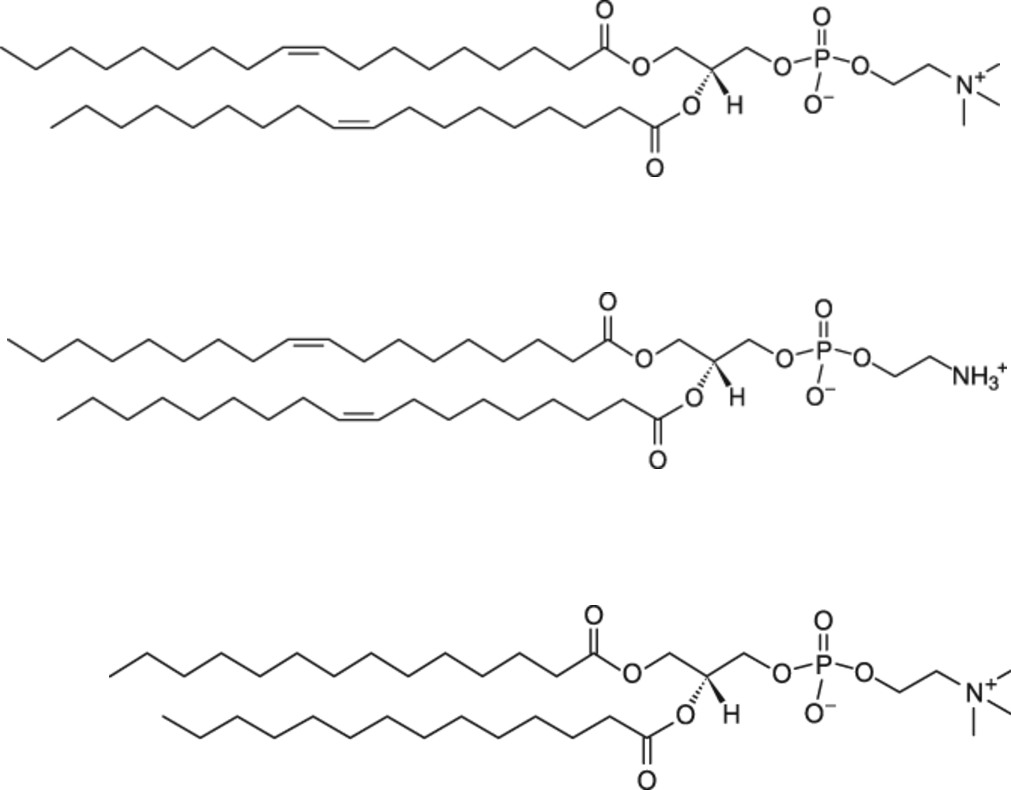
\includegraphics[width=0.5\textwidth]{figures/lipid_structure}
  \caption{Lipid structures of DOPC (top), DOPE (middle),
  and DMPC (bottom). Images are from Avanti Polar Lipids.}
  \label{fig:lipid_structure}
\end{figure}

\section{Tat peptide}\label{sec:Tat_peptide}
A protein important for infection is produced by the HIV Tat regulatory gene.
After synthesis on the HIV RNA, Tat protein enters a cell's nucleus where it is a
transcriptional transactivator for the long terminal repeat (LTR)
promoter which acts by binding to the Tar RNA element \cite{Vaishnav91}
(Fig.~\ref{fig:HIV_lifecycle}).
More recently, it was discovered that Tat participates in RNA
initiation by stimulating the transcription complex \cite{Raha05}.
Both of these roles activate the HIV virus and increase viral loads.
One focus of current AIDS research is to eradicate reservoirs of 
infected memory T-cells that contain dormant HIV;
Tat can awaken latent provirus \cite{Macias09}.
An understanding of Tat transport could lead to new or more effective 
HIV treatments. Tat could be prevented from
reaching the nuclear genome. Tat could awaken dormant virus so that
it can be targeted by standard treatments that only
work on active virus \cite{Macias09}. 

Of the 86 amino acids in Tat,
the highly basic (Y$_{47}$GRKKRRQRRR$_{57}$) sequence called Tat peptide 
is essential to transport
Tat through the nuclear membrane \cite{Ruben89,Hauber87}. 
Mutations within
this region yield a Tat protein that does not penetrate the cell 
nucleus. Tat peptide membrane translocation efficiency 
has made it a model for peptide-aided protein and drug delivery
\cite{Futaki01}. 
The mechanism of Tat-peptide translocation of proteins, 
DNA, RNA, and drugs across the membrane is of considerable interest
since it is known that desolvating and moving charged groups across membranes
can be energetically prohibitive \cite{Grabe04}. 
It has been suggested by MD simulations that Tat peptide first binds rather
more deeply in the membrane, below the phosphates, than
would be anticipated for such a highly charged peptide. From that position,
Tat may electrostatically attract the phosphates in the distal monolayer
leading to the formation of a transient water-filled pore through which
proteins and drugs diffuse \cite{Herce07}. 
We studied the transverse location of Tat within model lipid membranes 
by X-ray scattering
combined with MD simulations. This study is described in chapter 2.

\begin{figure}[htbp]
  \centering
  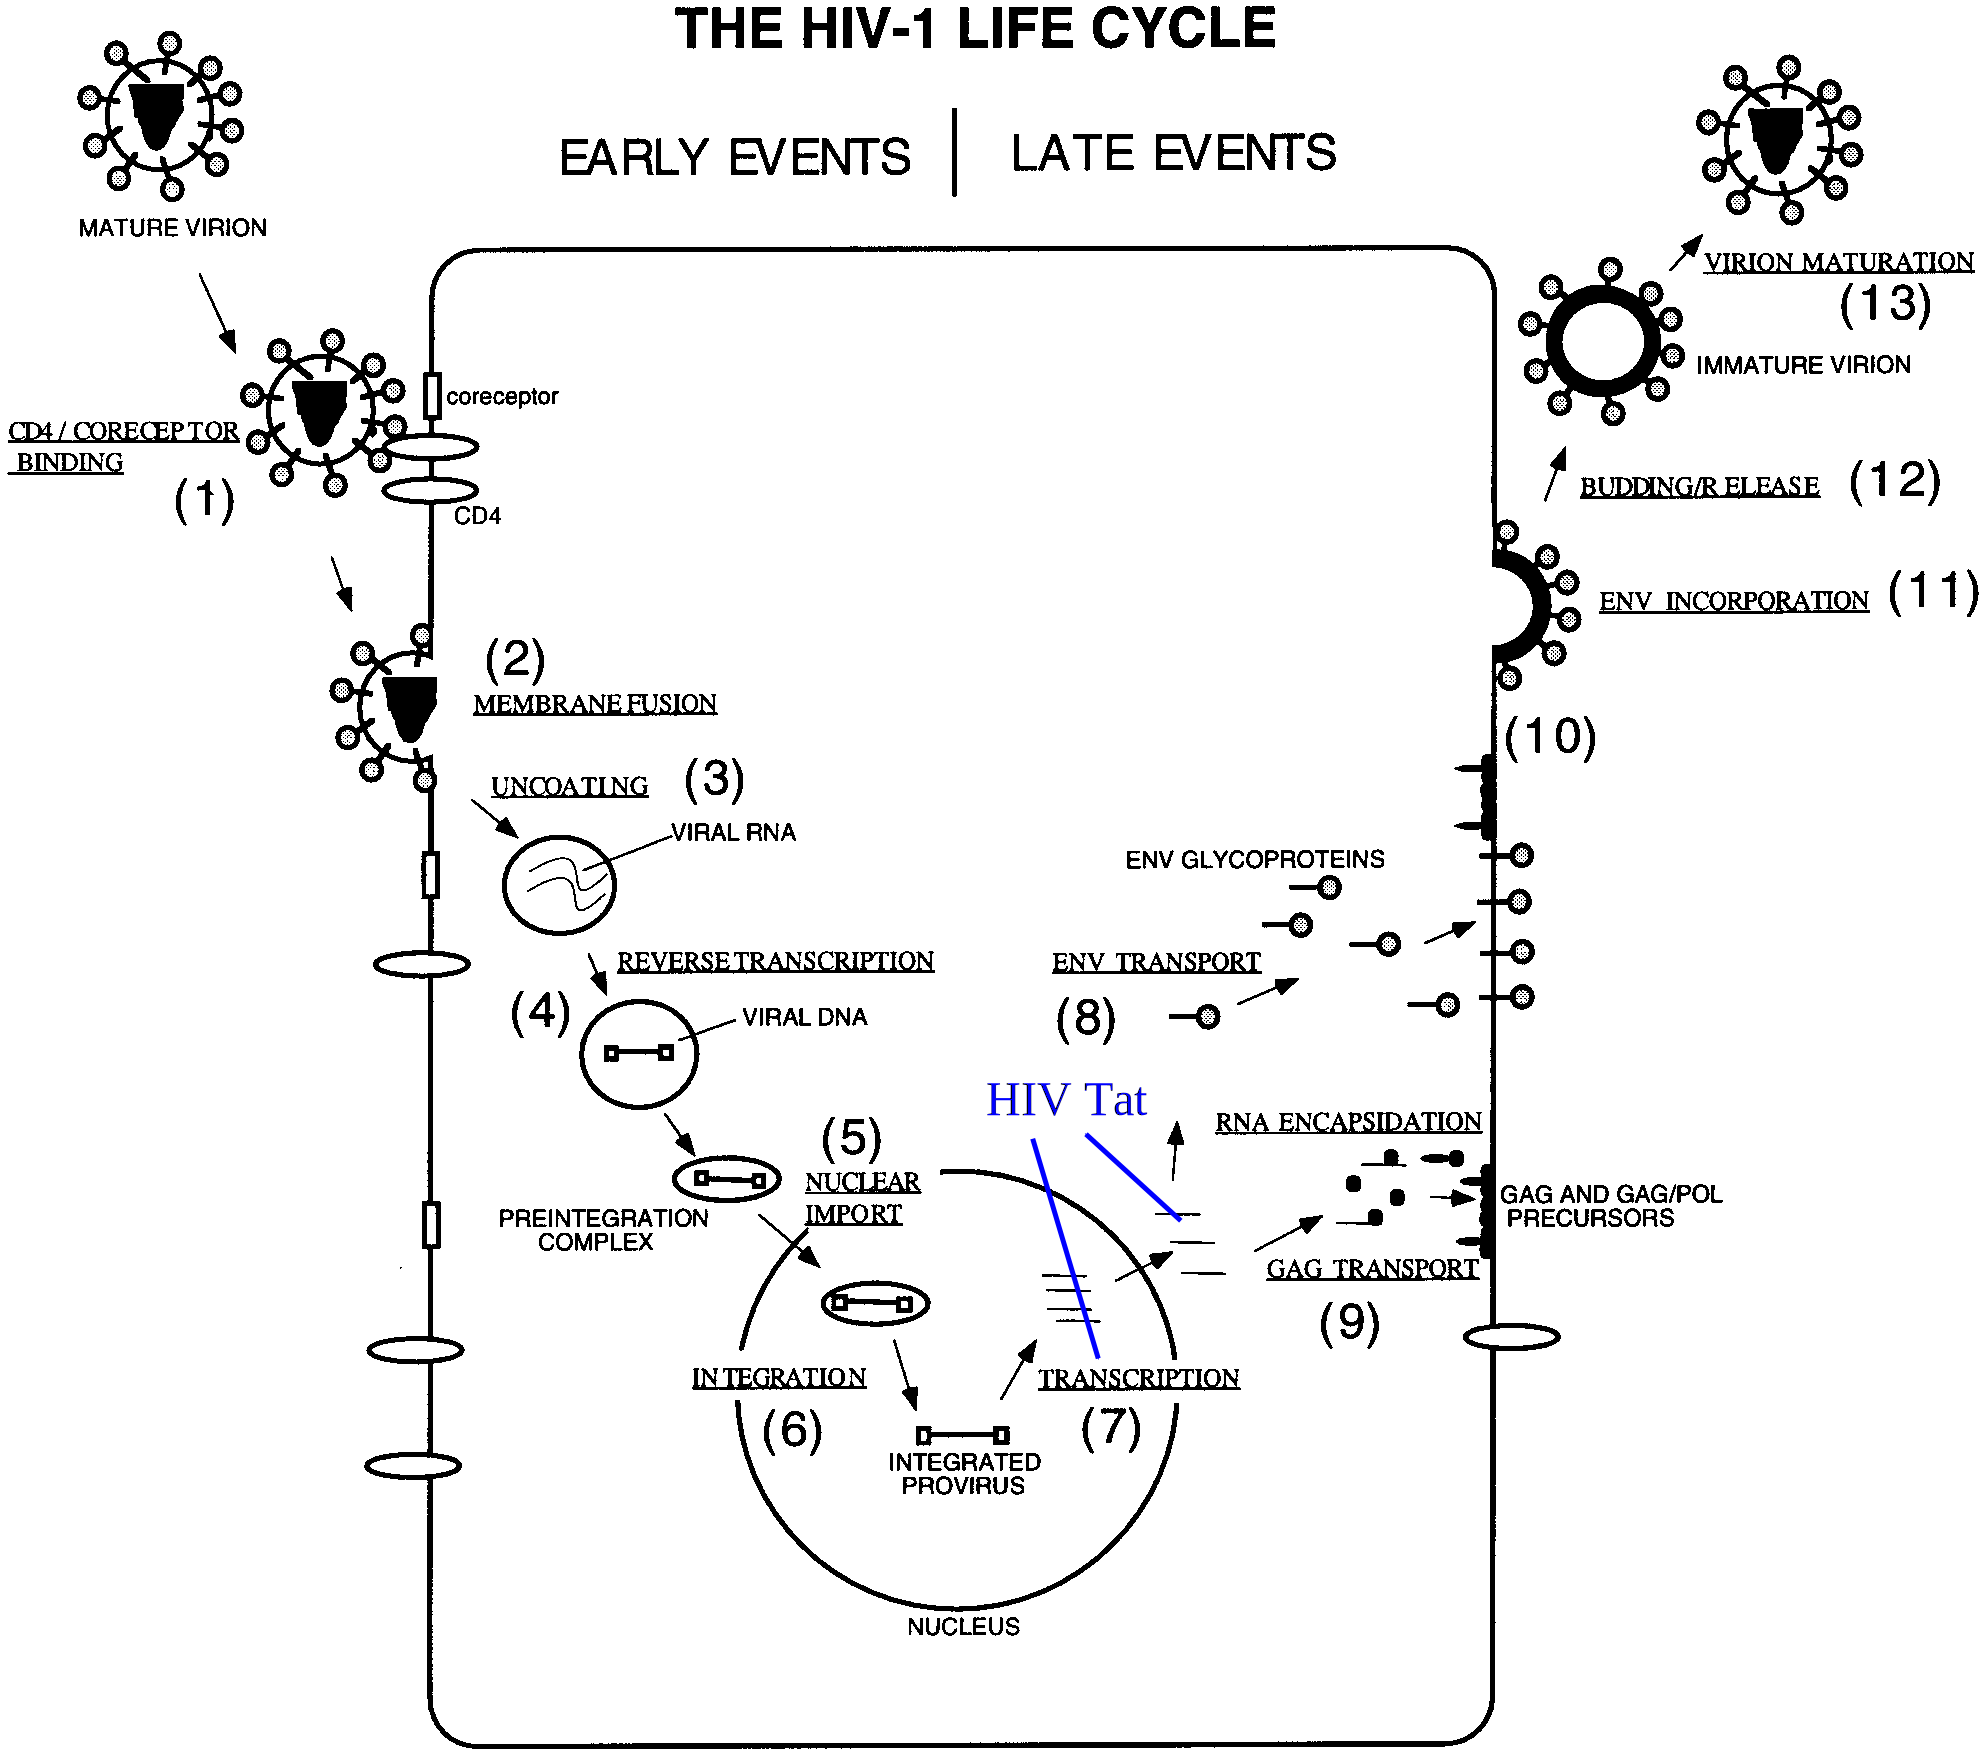
\includegraphics[width=\textwidth]{figures/HIV_lifecycle}
  \caption{HIV-1 life cycle, adapted from Ref.~\cite{Freed98}
  (additions in blue).}
  \label{fig:HIV_lifecycle}
\end{figure}

\section{$P_{\beta'}$ ripple phase}\label{sec:ripple_phase}
For some lipids, a height modulated phase where
bilayers are no longer flat exists between the fluid and gel phases
(Fig.~\ref{fig:phase_diagram}). 
This phase was termed $P_{\beta'}$ 
and is commonly called the ripple phase \cite{ref:Tardieu73}. 
The $P_{\beta'}$--$L_{\beta'}$ transition is often
called the pre-transition \cite{ref:Wack89} or lower transition \cite{Nagle00}.
The ripple phase has fascinated many researchers in condensed matter physics
and physical chemistry as an example of periodically modulated phases,
with many theoretical papers attempting to explain why there are 
ripples 
\cite{ref:Doniach79,ref:Marder84,ref:Hawton86,ref:Carlson87,ref:Goldstein88,ref:McCullough90,ref:Honda91,ref:Lubensky93,ref:Sengupta01,ref:Kamal11}
and a few simulation papers to shed light on molecular organization 
\cite{ref:deVries05,ref:Lenz07,ref:Scott84,ref:Debnath09}.
%From an accurate ripple structure, some indication of the energetcis of the ripple 
%formation may be obtained by comparing the relative size of the ripple wavelength
%and the ripple amplitude to the size of lipid molecules and the bilayer thickness 
%\cite{ref:Goldstein88}.
Despite many systematic studies over the past three decades
\cite{ref:Tardieu73,ref:Janiak76,ref:Copeland80,ref:Ruppel83,ref:Zasadzinski87,ref:Wack89,ref:Sun96,ref:Katsaras00,ref:Sengupta03}, 
molecular details of the structure are still lacking, which impedes
theoretical understanding of its origin.

Most studies have been performed on PCs, which readily form multilamellae
with definite interbilayer distance when dispersed in water \cite{Nagle00}.
PCs have a fairly bulky headgroup, creating a size mismatch with its acyl chains,
especially below the main phase transition. This is believed to be the 
reason why the acyl chains are tilted in the gel phase of PCs \cite{Nagle00,ref:Mcintosh80,ref:Nagle76}.
It has been proposed that the driving force for the ripple formation is also 
coupled to this size mismatch, with headgroup hydration playing an important role
\cite{ref:Cevc91,ref:Carlson87}.
It is not yet established whether the chains remain tilted in the ripple phase \cite{ref:Sun96}.

Generally, it is assumed that the lipids in the ripple phase are mainly in all-trans
configuration, as in the gel phase \cite{ref:Sengupta03}.
However, many studies point to the coexistence of fluid and gel regions
\cite{ref:Wittebort81,ref:Schneider83,ref:Sun96,ref:Marsh80,ref:Cunningham98,ref:Rappolt00}.
An X-ray structural study has reported that the ripples are composed of 
a longer sawtooth arm with characteristics similar to a gel phase bilayer 
and a shorter arm that is thinner and less densely packed\cite{ref:Sun96}, 
more compatible with a fluid phase bilayer or with a more recently proposed
interdigitated \LI\ phase.
Changes of bilayer packing along the ripple direction were also reported in
molecular dynamics simulations \cite{ref:deVries05}.
Yet, coexistence of different bilayer packing has not been established.
 
Studies of the ripple phase are normally done on multilamellar systems, but
some works have reported the existence of ripples in unilamellar vesicles
\cite{ref:Mason99,ref:Parente84}.
We studied the electron density distribution and chain packing 
of the asymmetric DMPC ripple phase formed by an oriented multilamellar sample
using synchrotron low and wide angle X-ray scattering.
Advantage of studying multilamellar systems with X-rays 
is intense, coherent out-of-plane diffraction peaks that lead to a detailed
bilayer structure \cite{ref:Sun96}.
Additionally, an oriented sample gives rise to even more intense diffraction peaks
compared to an unoriented sample. With careful analysis, high resolution
structure can be obtained.
An oriented sample also yields anisotropic
in-plane chain correlation scattering 
that can be analyzed to elucidate the molecular organization within 
the rippling bilayers, as was successfully done for the gel phase 
\cite{ref:Tardieu73,ref:Smith88,ref:Tristram93}.
Our aim was to study whether all-trans chains are tilted with respect to 
the bilayer normal and to elucidate the coexistence of different bilayer packing.
My ripple study is presented in chapter 3. 

%\begin{figure}[htbp]
%  \centering
%  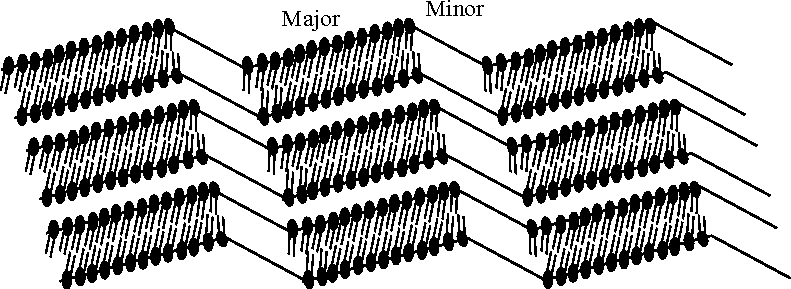
\includegraphics[width=0.7\textwidth]{figures/ripple_cartoon}
%  \caption{Schematic of the $P_{\beta'}$ ripple phase. In this phase, 
%  bilayers assume a periodic height modulation with a sawtooth shape.
%  The longer side of a sawtooth is called the major arm, and the shorter
%  side is called the minor arm. It is generally assumed that chains are
%  in an all-trans conformation in the major arm, but the molecular packing
%  in the minor arm is unknown.}
%  \label{fig:ripple_cartoon}
%\end{figure}